\documentclass{article}
\usepackage[parfill]{parskip}
\usepackage{amsmath,amssymb,amsthm}
\usepackage{a4wide}
\usepackage{color}
\usepackage{graphicx}
\graphicspath{{./images/}}
\usepackage[english]{babel}
\usepackage{authblk}

\renewcommand{\epsilon}{\varepsilon}
\newcommand{\bigo}[1]{\mathcal{O}\left(#1\right)}
\newcommand{\note}[1]{\emph{\color{blue}#1}.\\}
\renewcommand{\L}{\mathcal{ L}}
\newcommand{\R}{\mathbb{ R}}
\let\div\relax
\DeclareMathOperator{\div}{div}
\title{Numerical Homogenization}\author[1]{Ivar Stefansson} 
\author[2]{Omar Richardson} 
\affil[1]{Department of Mathematics and Computer Science, Karlstad University} 
\affil[2]{Department of Mathematics, University of Bergen} 


\begin{document}
\maketitle
\section{Project aim}
\label{sec:project_aim}

We aim to compute effective parameters of a composite material numerically using a finite element simulation implemented in FeNiCS.
Our goal is to explore the relations between the finite element mesh size and the variation in material data.
We consider the Poisson equation with a rapid variation in the diffusion coefficient and explore different solution techniques, focusing in particular on convergence rates and stability.

\section{Model}
\label{sec:model}
We consider a diffusion problem in a composite material. We denote the (periodic) domain with $\Omega \subset \R^d$, for $d\in\{1,2,3\}$. Within this material, we consider unknown quantity $u(x)$, of which the distribution is given by the solution of the Poisson equation:
\begin{equation}
    \begin{split}
        -\nabla \cdot (A_\epsilon(x)\nabla u(x)) &= f(x) \mbox{ for } x \in \Omega,\\
        u(x) &= 0 \mbox{ for } x \in \partial\Omega.
    \end{split}
    \label{eq:model}
\end{equation}

Here, $\epsilon$ is a small positive parameter, denoting the rapid variation of the material.
For diffusivity $A_\epsilon(x)$, we choose a periodic function with a period of order $\epsilon$, like
$$$$
\begin{equation}
   A_\epsilon(x) = \left( 2+\cos\left(\frac{2\pi x}{\epsilon}\right) \right)^{-1}.
   \label{eq:diff_param}
\end{equation}
For $\epsilon \to 0$, it is possible to obtain an homogenized diffusivity, called 'effective diffusion coefficient'.
If time permits, we will extend the model with a diffusion coefficient also varying in the normal length scale, and finally include time dependence in the model as well.

\section{Approximation with FeNiCS}
\label{sec:one_dim_approx}

We implement \eqref{eq:one_dim} in FeNiCS by providing the weak form
\begin{equation}
    \int_\Omega A_\epsilon\nabla u\nabla\phi dx= \int_\Omega f\phi dx
\end{equation}
where $\phi$ is a test function in $H^1_0(\Omega)$. We use second order Lagrangian basis functions on an evenly spaced unit interval mesh to find the weak solution.
An illustration of the numerical approximation is shown in Figure~\ref{fig:one_dim_approx}. 

\begin{figure}[ht]
    \centering
    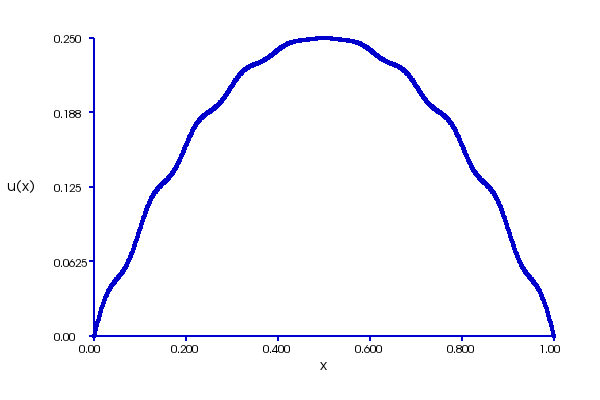
\includegraphics[width=0.5\linewidth]{one_dim_approx.png}
    \caption{Result of FeNiCS simulation of \eqref{eq:one_dim} for $\epsilon=0.1$ and $h = 1/80$}
    \label{fig:one_dim_approx}
\end{figure}

\begin{figure}[ht]
    \centering
    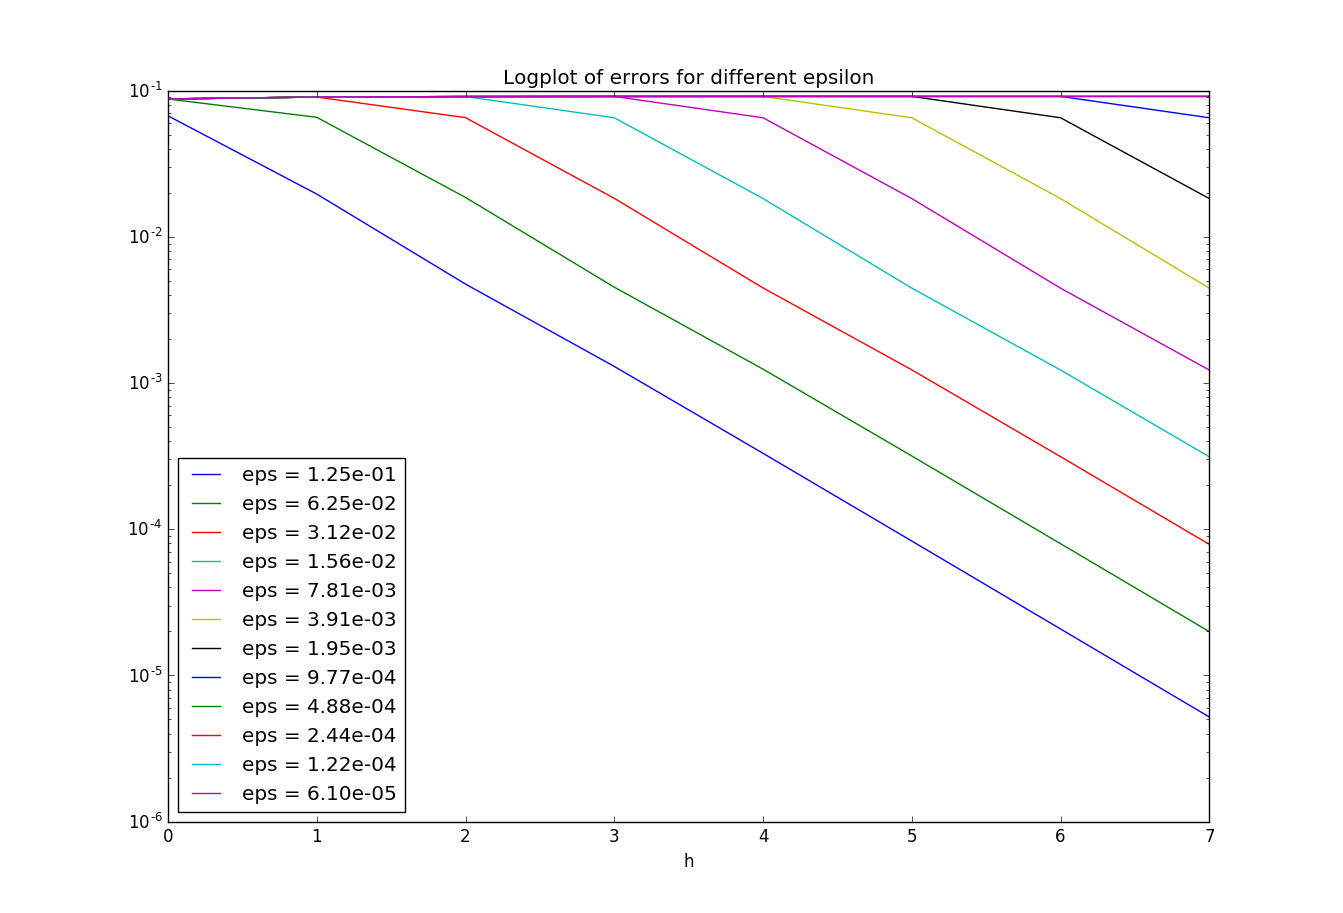
\includegraphics[width=0.5\linewidth]{one_dim_h_eps1.png}
    \caption{Logarithmic plot of error norms for $h\to 0$, several values of $\epsilon$.}
    \label{fig:one_dim_h_eps1}
\end{figure}

\begin{figure}[ht]
    \centering
    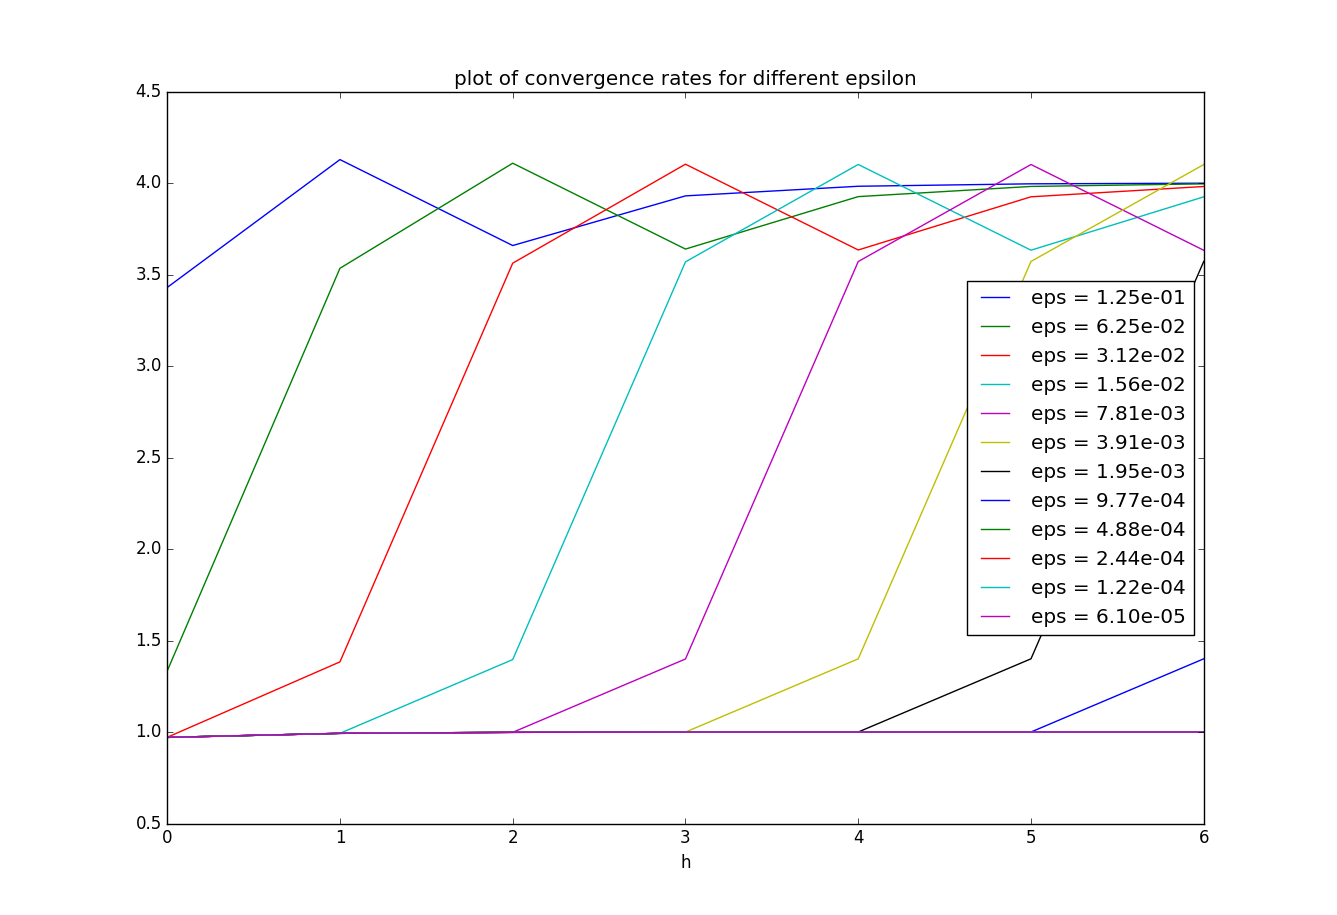
\includegraphics[width=0.5\linewidth]{one_dim_h_eps2.png}
    \caption{Plot of convergence rates, several values of $\epsilon$.}
    \label{fig:one_dim_h_eps2}
\end{figure}

\section{One-dimensional illustration}
\label{sec:onedim}
Let $A_\epsilon$ be defined as in \eqref{eq:diff_param}, let $f(x) = 1$ and let $\Omega = [0,1]$. For this particular choice, we are able to compute the solution to \eqref{eq:model} exactly, since it reduces to :
\begin{equation}
    \left( \frac{u'(x)}{2+\cos \left( \frac{2\pi x}{\epsilon} \right)} \right)' = 1
    \label{eq:one_dim}
\end{equation}

Integrating the left hand side of \eqref{eq:one_dim}, dividing by $A_\epsilon$, integrating by parts and substituting the Dirichlet boundary condition yields
\begin{equation}
    u(x) = \left( \frac{1}{2} - x \right) \left(2x + \frac{\epsilon}{2\pi}\sin\left(\frac{2\pi x}{\epsilon}\right) \right) + \frac{\epsilon^2}{(2\pi)^2}\left( 1 - \cos \left( \frac{2\pi x}{\epsilon} \right) \right) + x^2
   \label{eq:one_dim_sol}
\end{equation}

\begin{figure}[th]
    \centering
    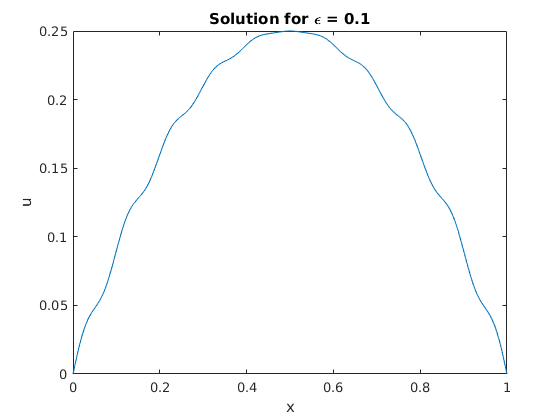
\includegraphics[width=0.5\linewidth]{one_dim_exact.png}
    \caption{Plot of the exact solution to \eqref{eq:one_dim} for $\epsilon=0.1$.}
    \label{fig:one_dim_exact}
\end{figure}

Figure~\ref{fig:one_dim_exact} presents the solution $u$ for $\epsilon = 0.1$. We observe oscillations of frequency $\bigo{1/\epsilon}$.

From \eqref{eq:one_dim_sol} we can induce that for $\epsilon \to 0$, the frequency of oscillations increases, but their amplitude decreases. This indicates that solving the equation with diffusivity $\lim_{\epsilon\to 0}A_\epsilon$ results in a smooth solution.

In Figure~\ref{fig:one_dim_h_eps1}, we see that for any $\epsilon$, convergence to the exact solution only occurs for $h \lesssim \epsilon$. Once this grid size restriction is satisfied, we obtain second order convergence as usual. Figure~\ref{fig:one_dim_h_eps2} presents this more clearly.

\section{Homogenization in higher dimensions}
Now, let $\Omega \subset [0,1]^d$ for $d=2,3$. We extend $A_\epsilon$ to multiple dimensions:
\begin{equation}
    A_\epsilon(x) =  \left( 2+\cos\left(\frac{2\pi \sum_{i=1}^dc_ix_i}{\epsilon}\right) \right)^{-1}
\end{equation}
where $c_i \in \R$ are arbitrary coefficients. 

Let $i,j=1,\dots,d$. Let $e_i$ be the $i$th basis vector of $\R^d$. To find the effective diffusion coefficient matrix $(A^*)_{ij}$, we solve the corresponding cell problems: find $w_i$ such that
\begin{equation}
    \begin{split}
        -\div_y(A(y)(e_i) + \nabla_y w_i(y)) = 0
    \end{split}
    \label{eq:cell_problem}
\end{equation}
where $w_i$ are periodic in $Y$.
We solve \eqref{eq:cell_problem} in FeNiCS. Its weak formulation is straightforward: find $w_i$ such that
\begin{equation}
    A(y)\nabla_y w_i \nabla_y \phi = \div_y(A(y)e_i)\phi
    \label{eq:weak_cell_problem}
\end{equation}
holds for all $\phi \in H^1_0(Y)$. We use once more second order Lagrangian basis functions, this time on a unit square or cube.
From the solution of \eqref{eq:cell_problem}, we obtain the diffusion coefficient by evaluating the following expression

\begin{equation}
    A^*_{ij} = \int_Y(e_j + \nabla_y w_j)\cdot(e_i + \nabla_y w_i)dy
    \label{eq:eff_diff}
\end{equation}

To find $A^*_{ij}$ in FeNiCS, we project the integrand of \eqref{eq:eff_diff} on the same function space as \eqref{eq:weak_cell_problem} and numerically integrate the result over $Y$.

Below follows an example for specific $A_\epsilon$, with $c_1=1$, $c_2=2$, $\epsilon = 0.25$ (see Figure~\ref{fig:two_dim_diff}).

\begin{figure}[h]
    \centering
    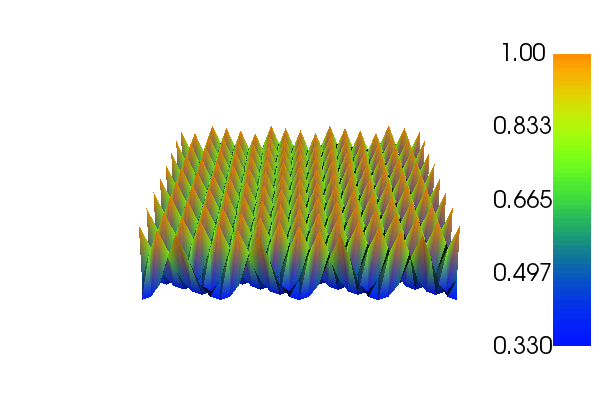
\includegraphics[width=0.8\linewidth]{two_dim_diff.png}
    \caption{Two dimensional diffusion coefficient $A_\epsilon$}
    \label{fig:two_dim_diff}
\end{figure}

Figure~\ref{fig:two_dim_approx} shows the corresponding solution of \eqref{eq:model}.
By solving the cell problems from \eqref{eq:cell_problem},  we obtain $A^*$ with values:
\begin{equation}
    A^* \approx \begin{bmatrix}
        1.024 & 0.047\\
        0.047 & 1.095
    \end{bmatrix}
\end{equation}
Finally, solving \eqref{eq:model} substituting $A_\epsilon$ with $A^*$ yields the result depicted in Figure~\ref{fig:two_dim_homog_approx}.
\begin{figure}[h]
    \centering
    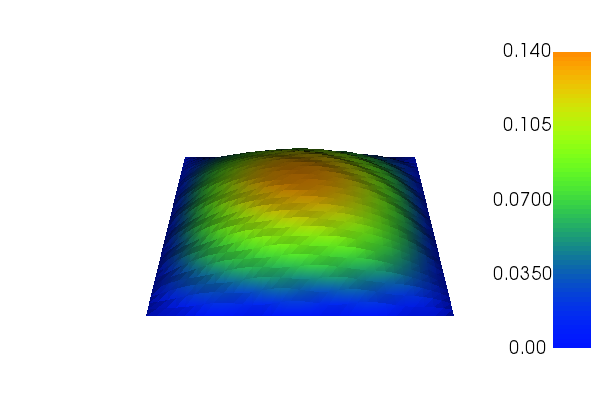
\includegraphics[width=0.8\linewidth]{two_dim_approx.png}
    \caption{Approximation of \eqref{eq:model} with $A_\epsilon$ as in Figure~\ref{fig:two_dim_diff}}
    \label{fig:two_dim_approx}
\end{figure}
\begin{figure}[h]
    \centering
    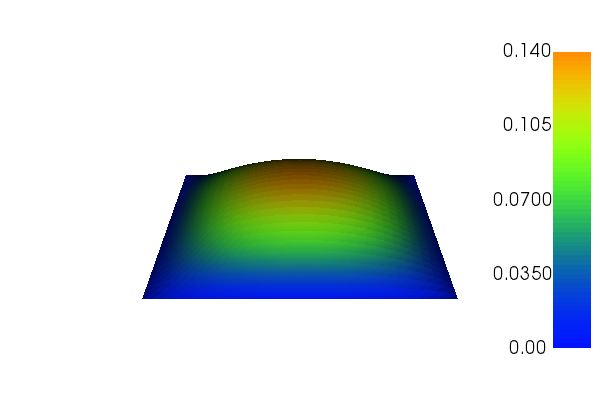
\includegraphics[width=0.8\linewidth]{two_dim_homog_approx.png}
    \caption{Homogenized approximation of \eqref{eq:model}.}
    \label{fig:two_dim_homog_approx}
 \end{figure}

 In the multi-dimensinal case, we are no longer able to compute an analytical solution. Therefore, we will henceforth evaluate our homogenized results by comparing them to a non-homogenized solution computed on a fine mesh. As shown in Section~\ref{sec:onedim}, the reference solution must resolve the spatial variation in $\epsilon$. With finite computer memory, this puts a restriction on the $\epsilon$ range we can investigate of roughly
\begin{equation}
    (\frac{10}{\epsilon})^d\leq C_{max}(Element).
    \label{eq:computational_restriction}
  \end{equation}
  Here, $C_{max}(Element)$ is the maximum number of cells the computer handles for a given choice of finite elements and the factor 10 ensures resolution of $\epsilon$.
  
  Let us now investigate the effect on the final problem solution of the spatial resolution in the cell problem solution. To do this, we solve the cell problem with a range of cell sizes $h_{cell,j}$ and use the obtained $A_{*,j}$ to compute homogenized global solutions. Then, we compute reference solutions as described in the previous paragraph for a range of $\epsilon_i$ which we compare the homogenized solutions to.

  The result is displayed in Figure~\ref{fig:two_dim_cell_problem_errors}. It shows that for large $h_{cell}$, the error is dominated by the inaccuracy in the $A_{*}$ computation. As the mesh size is decreased, the error converges to a value dominated by a combination of the homogenization approximation and the error in the computation of the homogenized solution, i.e., related to the mesh size of the global solution, $h_{global}$. The former of these two decreases in $\epsilon$, as can be seen from the fact that each line of the figure lies beneath all lines corresponding to higher values of $\epsilon$. The second one is assumed to be negligible for this parameter range, as the global homogenized problem was solved with considerably higher accuracy than the cell problem ($h_{global}=\frac{1}{2^7}$).
  We note that the error does not decrease monotonically in $h_{cell}$, but rather increases going from $2 \times 2$ to $4 \times 4$ cells. While we are not entirely sure about the reason for this, one possible explanation could be that the 2 by 2 grid is somehow favourably aligned with $A_{\epsilon}$. We note, however, that for this $\epsilon$ range, the error seems to converge for $h_{cell}\leq 1dsjkl$. Consequently, we will use this value in the following and assume that the cell problem error is negligible.

  \begin{figure}[h]
    \centering
    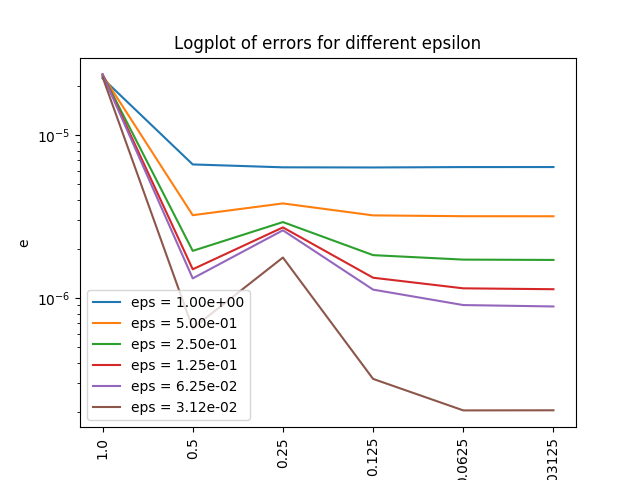
\includegraphics[width=0.8\linewidth]{2d_cell_errors.png}
    \caption{Errors as a function of cell problem discretization size $h_{cell}$ for various $\epsilon$ values.}
    \label{fig:two_dim_cell_problem_errors}
 \end{figure}

 Now, we explore the convergence in the global mesh size $h_{global}$ of the homogenized solution for different values of $\epsilon$. We proceed as above, except that we keep fix $h_{cell}=1dslkf$ and vary  $h_{global}$. Figure~\ref{fig:two_dim_global_problem_errors} shows how an initial decrease before the error stagnates. The $\epsilon$ variation in the limit value shows the convergence of the homogenization model for $\epsilon\to 0$. This is of particular interest, since it validates that the homogenized solution approaches the full one as $\epsilon$ to   See also Figure~\ref{fig:two_dim_global_problem_errors} for the convergence rates of this case.
   \begin{figure}[h]
    \centering
    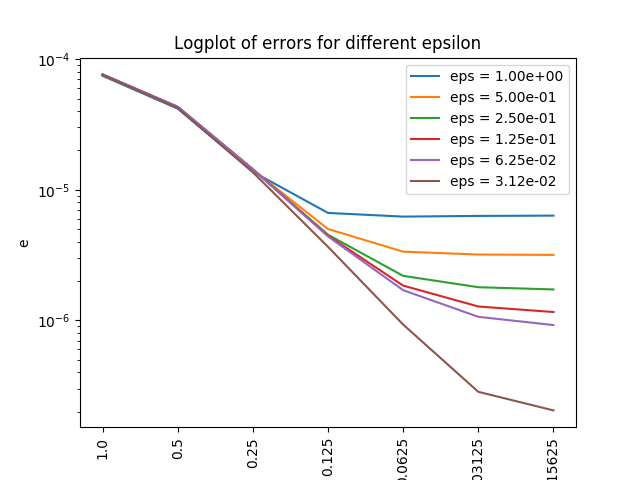
\includegraphics[width=0.8\linewidth]{2d_global_errors.png}
    \caption{Errors as a function of cell problem discretization size $h_{cell}$ for various $\epsilon$ values.}
    \label{fig:two_dim_global_problem_errors}
  \end{figure}
   \begin{figure}[h]
    \centering
    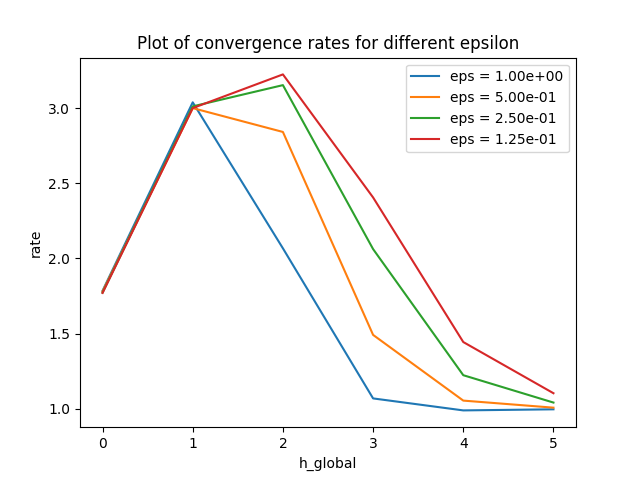
\includegraphics[width=0.8\linewidth]{2d_global_rates.png}
    \caption{Convergence rates as the global discretization size $h_{cell}$ approaches zero for various $\epsilon$ values.}
    \label{fig:two_dim_global_problem_rates}
  \end{figure}

  \subsection{Complex domains}\label{sec:car}
  In this section, we briefly investigate the possibilities of FEniCS offers for more complicated domains. To this end, we set up a somewhat more demanding domain geometry. We again perform simulations for different $\epsilon$ values (Figures~\ref{fig:car_reference_0} and \ref{fig:car_reference_3}) to the homogenized solution displayed in Figure~\ref{car_homogenized}. The computational parameters are listed in Table~\ref{tab:car_values}. Using fine meshes for both the cell and global problem, we can again investigate the convergence for decreasing $\epsilon$. The errors of the homogenized solution compared to the full one for each $\epsilon$ are plotted in Figure~\ref{}, and seem to validate the convergence in the limit. The slight reduction in convergence rate observed for the smaller $\epsilon$ is assumed to be due to errors caused by the finitude of $h_{cell}$ and $h_{global}$. 
  

  \begin{figure}[h]
    \centering
    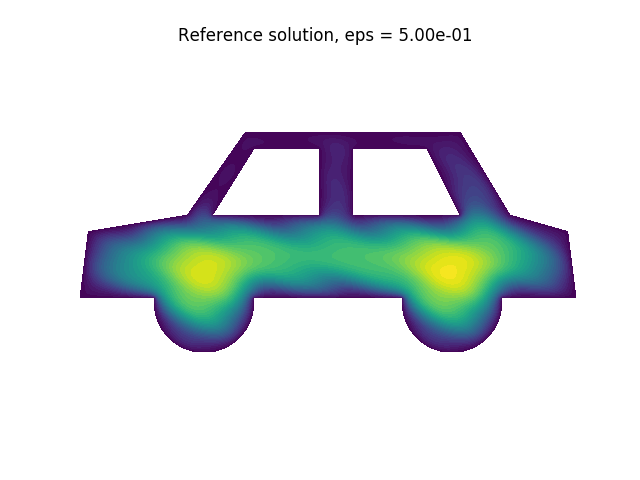
\includegraphics[width=0.8\linewidth]{carw_reference_eps_power_1.png}
    \caption{Solution of the Poisson problem on a cartoon car domain for $\epsilon = \frac{1}{2}$.}
    \label{fig:car_reference_1}
  \end{figure}
  \begin{figure}[h]
    \centering
    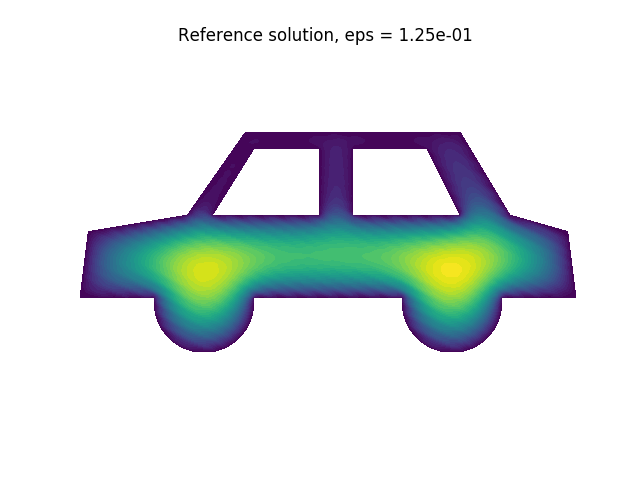
\includegraphics[width=0.8\linewidth]{carw_reference_eps_power_3.png}
    \caption{Solution of the Poisson problem on a cartoon car domain for $\epsilon = \frac{1}{2^3}$.}
    \label{fig:car_reference_3}
  \end{figure}
  \begin{figure}[h]
    \centering
    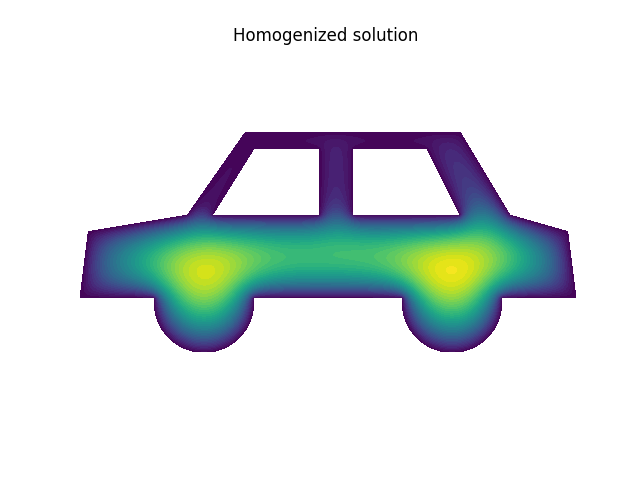
\includegraphics[width=0.8\linewidth]{carw_homogenized.png}
    \caption{Homogenized solution of the Poisson problem on a cartoon car domain.}
    \label{fig:car_homogenized}
  \end{figure}
   \begin{figure}[h]
    \centering
    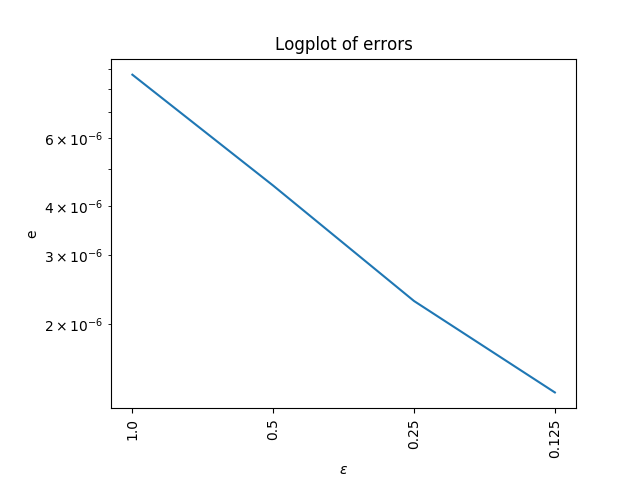
\includegraphics[width=0.8\linewidth]{carw_errors.png}
    \caption{Errors of the homogenized solution for $\epsilon \in [\frac{1}{2^3}, 1]$.}
    \label{fig:car_errors}
  \end{figure}
  
  \section{Solvers and preconditioners}
  We now present a short study of the performance of different linear solver schemes and preconditioners for this Poisson type problem. We have chosen a subset of the available FEniCS options. The solver methods are Conjugate gradients (cg), Generalized minimal residual (gmres), Minimal residual (minres) and Biconjugate gradient stabilized (bicgstab) and the preconditioners Incomplete Cholesky factorization (icc), Incomplete LU factorization (ilu),  Jacobi iteration (jacobi), Successive over-relaxation (sor) and finally without any preconditioner (none). We have solved both the homogenized and the full problem with two different $h_{global}$ values, whereof the first ($\frac{1}{2^3}$) leads to a small, assumedly quite manageable problem, whereas the second ($\frac{1}{2^7}$) may pose a somewhat larger challenge.
  The first observation is that using the Incomplete Cholesky factorization, the cg and minres fail to converge even for small problems. Convergence is maintained for the gmres and bicgstab also for the larger problem, although at rather poor computational times, see Figures~\ref{fig:solution_times_icc_big_h} and~\ref{fig:solution_times_icc_small_h}. The results from the rest of the simulations are presented in Figures~\ref{fig:solution_times_full_big_h} through \ref{fig:solution_times_homogenized_small_h}. We note that in general, there is less to tell the choices apart for the smaller problem. As expected, the absolute computing times are also much smalller, reducing even further our interest in those number.

  Focusing now on the larger system (Figures \ref{fig:solution_times_full_small_h} and \ref{fig:solution_times_homogenized_small_h}), the trend is that it pays off to use a preconditioner compared to solving without any (none). It also seems that the ilu is a good choice for larger Poisson problems, and that one might want to avoid using the gmres.

  Finally, we include the same data for the full problem on an even finer mesh ($h_{global}=\frac{1}{2^9}$). It shows the same general trends as on the mesh just discussed, with the exception that gmres now fails to converge at all both with the jacobi preconditioner and without preconditioning, see Figure~\ref{fig:solution_times_full_tiny_h}. 
%  \begin{tabular}[c]{l | c c c c}
%     & cg & gmres & minres & bicgstab \\
%    \hline
%    none&  &  &  &  \\
%    sor&  &  &  &  \\
%    ilu&  &  &  &  \\
%    jacobi&  &  &  &  \\
%    \title{Computational times for different solver and preconditioner combinations}
     %      \label{tab:solvers_and_preconditioners}
\begin{figure}[h]
    \centering
    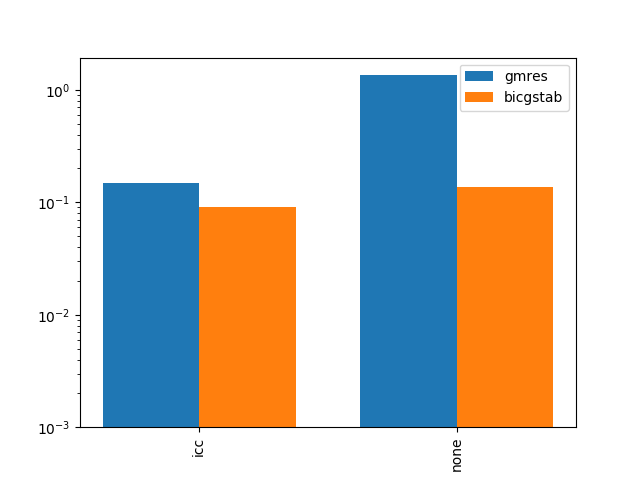
\includegraphics[width=0.8\linewidth]{solution_times_icc_big_h.png}
    \caption{Computation times for the non-homogenized problem and coarse mesh using the gmres and bicgstab solvers and no and icc preconditioning.}
    \label{fig:solution_times_icc_big_h}
  \end{figure}
  \begin{figure}[h]
    \centering
    \includegraphics[width=0.8\linewidth]{}%{solution_times_icc_small_h.png}
    \caption{Computation times for the non-homogenized problem and fine mesh using the gmres and bicgstab solvers and no and icc preconditioning.}
    \label{fig:solution_times_icc_small_h}
  \end{figure}
  
  % Perhaps the following results should rather be presented in tables or as bar charts or something?
  \begin{figure}[h]
    \centering
    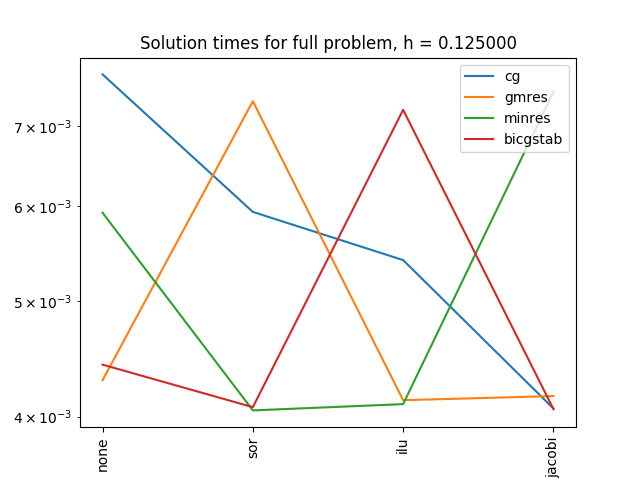
\includegraphics[width=0.8\linewidth]{solution_times_full_big_h.png}
    \caption{Computation times for the non-homogenized problem and coarse mesh using different solver-preconditioner combinations.}
    \label{fig:solution_times_full_big_h}
  \end{figure}
  \begin{figure}[h]
    \centering
    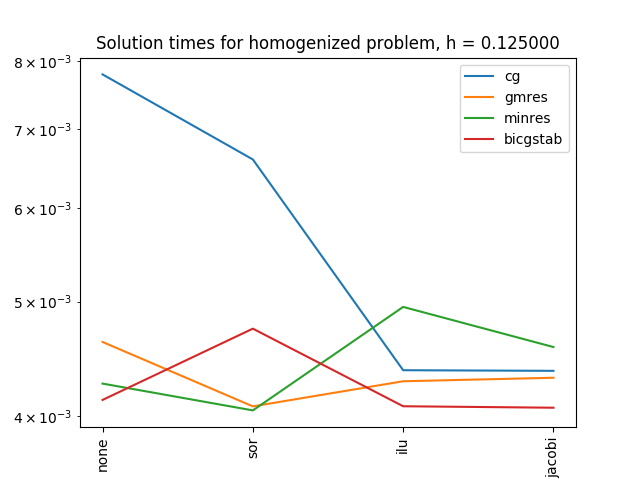
\includegraphics[width=0.8\linewidth]{solution_times_homogenized_big_h.png}
    \caption{Computation times for the homogenized problem and coarse mesh using different solver-preconditioner combinations.}
    \label{fig:solution_times_full_big_h}
  \end{figure}
  \begin{figure}[h]
    \centering
    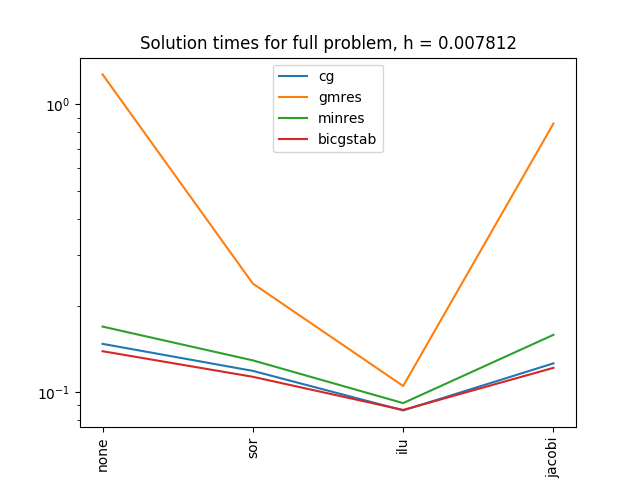
\includegraphics[width=0.8\linewidth]{solution_times_full_small_h.png}
    \caption{Computation times for the non-homogenized problem and fine mesh using different solver-preconditioner combinations.}
    \label{fig:solution_times_full_small_h}
  \end{figure}
  \begin{figure}[h]
    \centering
    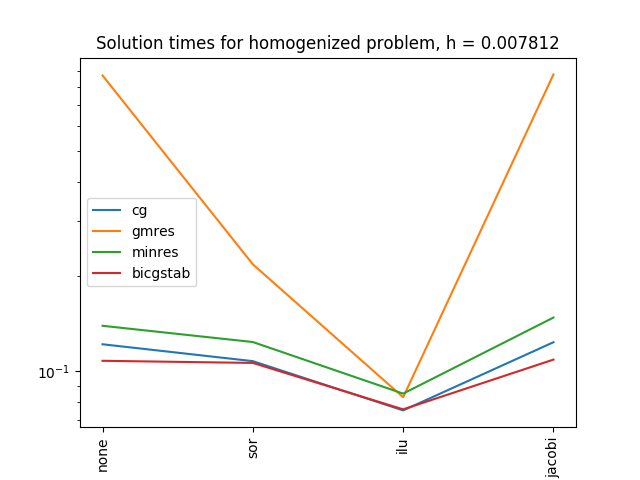
\includegraphics[width=0.8\linewidth]{solution_times_homogenized_small_h.png}
    \caption{Computation times for the homogenized problem and fine mesh using different solver-preconditioner combinations.}
    \label{fig:solution_times_full_small_h}
  \end{figure}
  \begin{figure}[h]
    \centering
    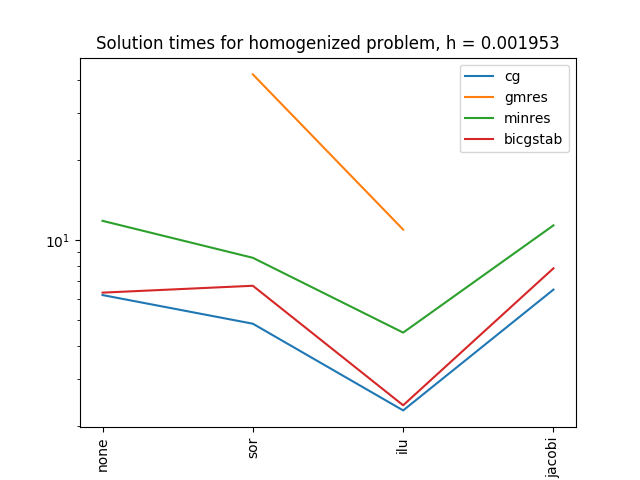
\includegraphics[width=0.8\linewidth]{solution_times_homogenized_tiny_h.png}
    \caption{Computation times for the homogenized problem and really fine mesh using different solver-preconditioner combinations.}
    \label{fig:solution_times_full_tiny_h}
  \end{figure}
\end{document}
